\documentclass[11pt,a4paper]{article}
\usepackage[utf8]{inputenc}
\usepackage[margin=0.8in]{geometry}
\usepackage{tikz}
\usetikzlibrary{shapes.geometric, arrows, positioning, calc, fit, backgrounds, shadows}
\usepackage{xcolor}
\usepackage{hyperref}
\usepackage{listings}
\usepackage{graphicx}
\usepackage{tcolorbox}
\usepackage{enumitem}
\usepackage{tabularx}
\usepackage{booktabs}
\usepackage{fancyhdr}
\usepackage{titlesec}
\usepackage{float}
\usepackage{amsmath}

% ============================================================================
% STYLING & COLORS
% ============================================================================
\definecolor{brandblue}{RGB}{33, 150, 243}
\definecolor{brandgreen}{RGB}{76, 175, 80}
\definecolor{brandorange}{RGB}{255, 152, 0}
\definecolor{brandpurple}{RGB}{156, 39, 176}
\definecolor{darkgray}{RGB}{66, 66, 66}
\definecolor{codebg}{RGB}{245, 245, 245}

% TikZ Styles
\tikzstyle{process} = [rectangle, rounded corners, minimum width=3cm, minimum height=1cm, text centered, draw=black, fill=brandblue!20, align=center, drop shadow]
\tikzstyle{decision} = [diamond, minimum width=2.5cm, minimum height=1cm, text centered, draw=black, fill=brandorange!30, aspect=2.5, font=\small, align=center, drop shadow]
\tikzstyle{sensor} = [ellipse, minimum width=2.5cm, minimum height=0.8cm, text centered, draw=black, fill=brandgreen!20, font=\small\bfseries, align=center, drop shadow]
\tikzstyle{action} = [rectangle, minimum width=2.5cm, minimum height=0.8cm, text centered, draw=black, fill=brandpurple!20, font=\small, align=center, drop shadow]
\tikzstyle{startstop} = [rectangle, rounded corners, minimum width=3cm, minimum height=1cm, text centered, draw=black, fill=brandgreen!40, drop shadow]
\tikzstyle{hardware} = [rectangle, rounded corners, minimum width=3cm, minimum height=1cm, text centered, draw=black, fill=brandorange!20, align=center, drop shadow]
\tikzstyle{motor} = [rectangle, minimum width=2.5cm, minimum height=0.8cm, text centered, draw=black, fill=red!20, align=center, drop shadow]
\tikzstyle{arrow} = [thick,->,>=stealth, rounded corners]

% Code Listing Style
\lstset{
    language=Java,
    backgroundcolor=\color{codebg},
    basicstyle=\ttfamily\small,
    keywordstyle=\color{brandblue}\bfseries,
    commentstyle=\color{brandgreen!70!black},
    stringstyle=\color{brandorange},
    numbers=left,
    numberstyle=\tiny\color{gray},
    frame=leftline,
    rulecolor=\color{brandblue},
    breaklines=true,
    tabsize=4,
    showstringspaces=false,
    captionpos=b
}

% Header/Footer
\pagestyle{fancy}
\fancyhf{}
\lhead{\textbf{Quanta Robotics}}
\rhead{Comprehensive Programming Portfolio}
\cfoot{\thepage}

% Title Formatting
\titleformat{\section}
{\color{brandblue}\normalfont\Large\bfseries}
{\color{brandblue}\thesection}{1em}{}

\titleformat{\subsection}
{\color{darkgray}\normalfont\large\bfseries}
{\thesubsection}{1em}{}

% ============================================================================
% DOCUMENT START
% ============================================================================
\begin{document}

% TITLE PAGE
\begin{titlepage}
    \begin{center}
        \vspace*{2cm}
        \includegraphics[width=4cm]{github_qr.png}\\[1cm]
        {\Huge \textbf{LYBOTICS QUANTA ROBOTICS}}\\[0.5cm]
        {\Large \textbf{Team Programming Portfolio}}\\[0.5cm]
        {\large Season: Decode Season (2025-2026)}\\[2cm]
        
        \textbf{\LARGE Comprehensive Technical Documentation}\\[1cm]
        
        \begin{tcolorbox}[colback=white, colframe=brandblue, title=\textbf{Abstract}]
            This document details the complete software architecture of the Quanta robot. It covers the distributed hardware control system, advanced sensor integration (IMU, Vision, Color), Finite State Machine (FSM) implementation, Closed-Loop Control algorithms, and Autonomous trajectory planning.
        \end{tcolorbox}
        
        \vfill
        
        \textbf{Table of Contents Highlights:}\\
        System Architecture \& Hardware Map\\
        Sensor Logic \& Algorithms\\
        Intelligent TeleOp \& Field-Centric Drive\\
        Autonomous Navigation \& Computer Vision\\
        Detailed Software Flowcharts
        
        \vfill
        
        {\large \today}
    \end{center}
\end{titlepage}

\tableofcontents
\newpage

% ============================================================================
% SECTION 1: SYSTEM OVERVIEW (CONTROL AWARD)
% ============================================================================
\section{System Architecture}

\subsection{Control System Implementation}
The Quanta Robot uses a distributed control architecture managed by the REV Control Hub. The system integrates three primary sensor modalities (Inertial, Vision, and Color) to drive automated actions in both TeleOp and Autonomous modes. 

\textbf{Key Innovation:} The integration of Dead Wheel Odometry (`par0`, `par1`, `perp`) allows for "Field-Centric" corrective steering during autonomous intake cycles, solving the problem of mechanical drift caused by uneven friction on the foam tiles.

\begin{center}
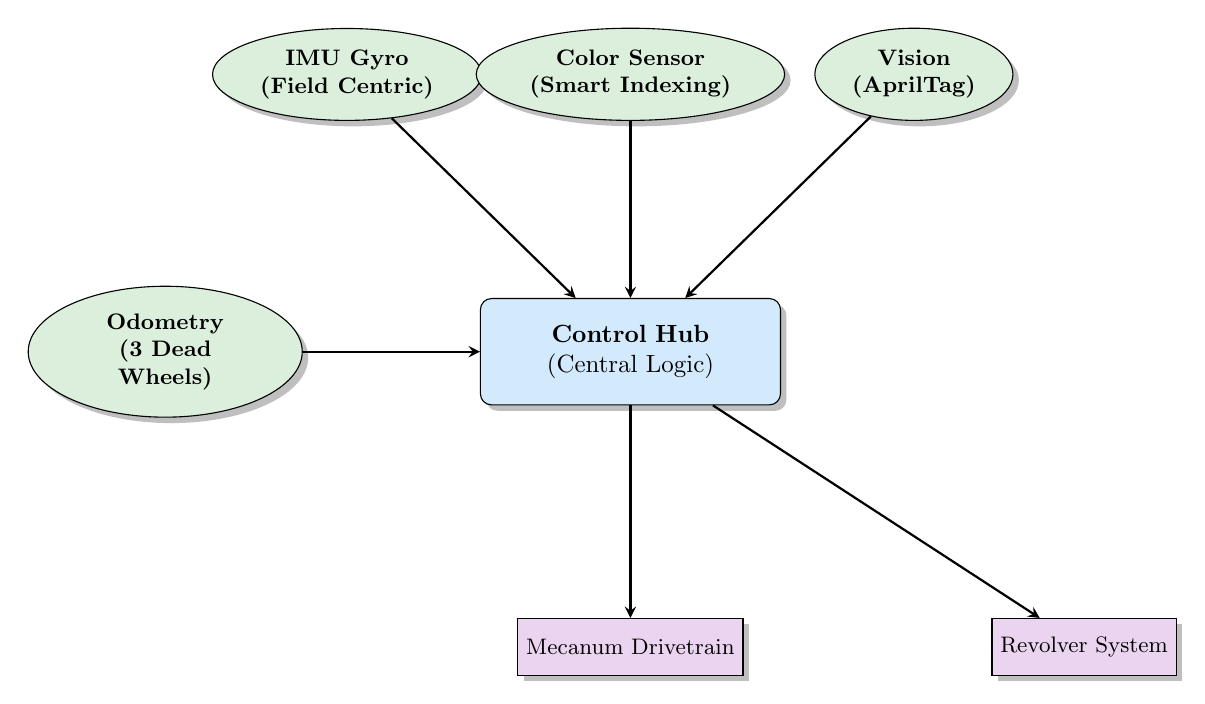
\begin{tikzpicture}[node distance=2.5cm, auto, scale=0.9, transform shape]
    % Central Controller
    \node (hub) [process, text width=4cm, minimum height=1.5cm] {\textbf{Control Hub}\\(Central Logic)};
    
    % Sensors (Top & Sides)
    \node (imu) [sensor, above=of hub, xshift=-4cm] {\textbf{IMU Gyro}\\(Field Centric)};
    \node (color) [sensor, above=of hub, xshift=0cm] {\textbf{Color Sensor}\\(Smart Indexing)};
    \node (vision) [sensor, above=of hub, xshift=4cm] {\textbf{Vision}\\(AprilTag)};
    
    % Dead Wheels
    \node (odo) [sensor, left=of hub, text width=2.5cm, align=center] {\textbf{Odometry}\\(3 Dead Wheels)};
    
    % Actuators (Bottom)
    \node (drive) [action, below=of hub, yshift=-0.5cm] {Mecanum Drivetrain};
    \node (revolver) [action, right=of drive, xshift=1cm] {Revolver System};
    
    % Arrows
    \draw [arrow] (imu) -- (hub);
    \draw [arrow] (color) -- (hub);
    \draw [arrow] (vision) -- (hub);
    \draw [arrow] (odo) -- (hub);
    \draw [arrow] (hub) -- (drive);
    \draw [arrow] (hub) -- (revolver);
\end{tikzpicture}
\end{center}

\subsection{Hardware Configuration Diagram}
We utilize a Control Hub and Expansion Hub configuration to manage our high actuator count.

\begin{center}
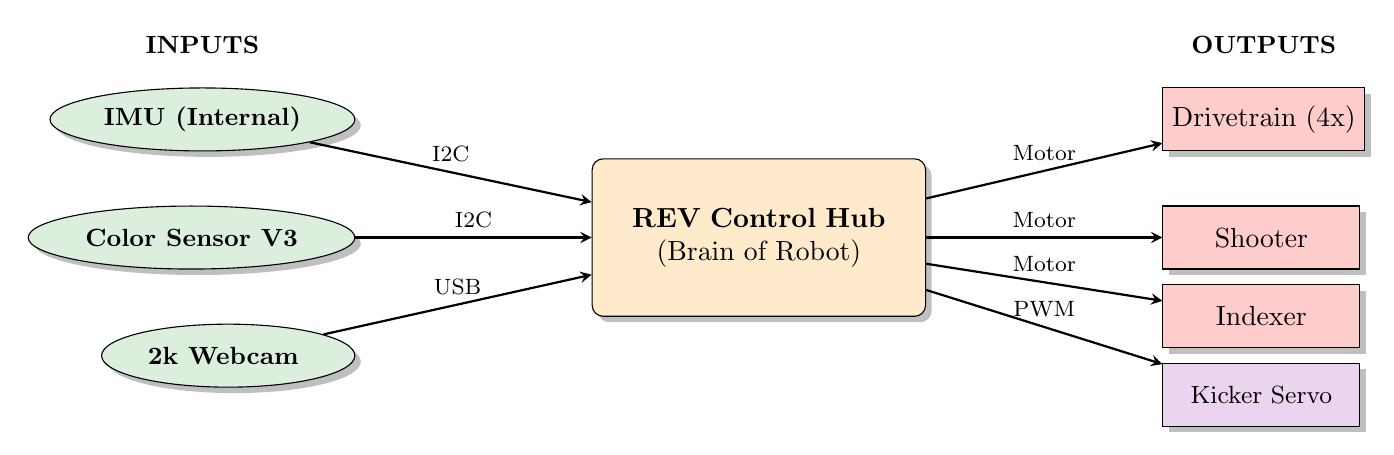
\begin{tikzpicture}[node distance=1.5cm, auto]
% Control Hub in center
\node (hub) [hardware, text width=4cm, minimum height=2cm] {\textbf{REV Control Hub}\\(Brain of Robot)};

% Sensors on the left
\node (imu) [sensor, left=3cm of hub, yshift=1.5cm] {IMU (Internal)};
\node (color) [sensor, left=3cm of hub, yshift=0cm] {Color Sensor V3};
\node (camera) [sensor, left=3cm of hub, yshift=-1.5cm] {2k Webcam };

% Motors on the right
\node (drive) [motor, right=3cm of hub, yshift=1.5cm] {Drivetrain (4x)};
\node (shooter) [motor, right=3cm of hub, yshift=0cm] {Shooter};
\node (indexer) [motor, right=3cm of hub, yshift=-1cm] {Indexer};
\node (kicker) [action, right=3cm of hub, yshift=-2cm] {Kicker Servo};

% Arrows from sensors to hub
\draw [arrow] (imu) -- node[above, font=\footnotesize] {I2C} (hub);
\draw [arrow] (color) -- node[above, font=\footnotesize] {I2C} (hub);
\draw [arrow] (camera) -- node[above, font=\footnotesize] {USB} (hub);

% Arrows from hub to motors
\draw [arrow] (hub) -- node[above, font=\footnotesize] {Motor} (drive);
\draw [arrow] (hub) -- node[above, font=\footnotesize] {Motor} (shooter);
\draw [arrow] (hub) -- node[above, font=\footnotesize] {Motor} (indexer);
\draw [arrow] (hub) -- node[above, font=\footnotesize] {PWM} (kicker);

\node[above=0.3cm of imu, font=\small\bfseries] {INPUTS};
\node[above=0.3cm of drive, font=\small\bfseries] {OUTPUTS};
\end{tikzpicture}
\end{center}

\subsection{Port Mapping Specification}
\begin{center}
\begin{tabular}{|l|l|l|l|}
\hline
\textbf{Component} & \textbf{Port} & \textbf{Signal} & \textbf{Description} \\
\hline
Left Front & Motor 0 & Encoder & Drivetrain + \textbf{Perp Dead Wheel} \\
Left Back & Motor 1 & Encoder & Drivetrain + \textbf{Par0 Dead Wheel} \\
Right Front & Motor 2 & Encoder & Drivetrain + \textbf{Par1 Dead Wheel} \\
Right Back & Motor 3 & Encoder & Drivetrain (Mecanum) \\
\hline
Shooter & Exp 0 & Encoder & Velocity PID Controlled \\
Indexer & Exp 1 & Encoder & Position PID (96 ticks/slot) \\
Intake & Exp 2 & Power & Continuous Rotation \\
\hline
Kicker & Servo 0 & PWM & Linear Actuator Simulation \\
\hline
\multicolumn{4}{|c|}{\textbf{Odometry Specification}} \\
\hline
\textbf{Name} & \textbf{Hub Port} & \textbf{Offset (Ticks)} & \textbf{Function} \\
\hline
\texttt{par0} & Motor 1 & -3820.67 (Y) & Parallel Tracking 1 \\
\texttt{par1} & Motor 2 & +3365.44 (Y) & Parallel Tracking 2 \\
\texttt{perp} & Motor 0 & -2005.03 (X) & Perpendicular Tracking \\
\hline
\end{tabular}
\end{center}

\newpage
% ============================================================================
% SECTION 2: INTELLIGENT ALGORITHMS
% ============================================================================
\section{Intelligent Algorithms \& Sensor Logic}

\subsection{Smart Indexing: Color Edge Detection}

\begin{tcolorbox}[colback=brandgreen!10, colframe=brandgreen, title=\textbf{Problem \& Solution}]
\textbf{Problem:} Manual indexing requires the driver to precisely time button presses while driving, leading to missed artifacts or jamming.
\textbf{Solution:} We implemented a Falling/Rising Edge Detector on the color sensor. The system triggers indexing ONLY when a valid color pattern (Green/Purple) transitions from "Not Detected" to "Detected".
\end{tcolorbox}

\textbf{Logic Flow:}
\begin{enumerate}
    \item \textbf{Filtering:} Calculate $Distance < 4cm$ AND $(Green > Threshold$ OR $Purple > Threshold)$.
    \item \textbf{State Memory:} Compare current state to previous loop state.
    \item \textbf{Action:} If `Current=Detected` and `Previous=Empty`, trigger Index Action.
\end{enumerate}

\begin{center}
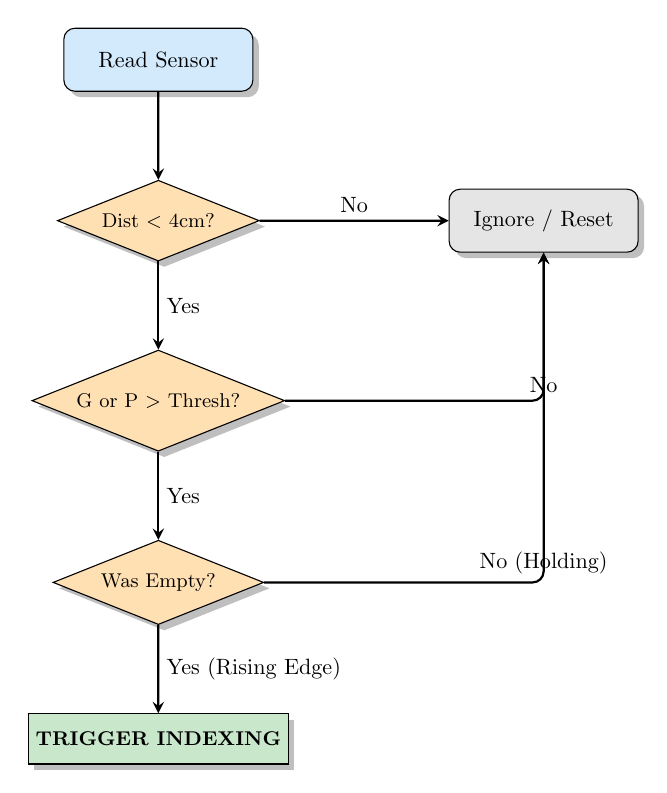
\begin{tikzpicture}[node distance=1.4cm, auto, scale=0.8, transform shape]
    \node (read) [process] {Read Sensor};
    \node (dist) [decision, below=of read] {Dist $<$ 4cm?};
    \node (color) [decision, below=of dist] {G or P $>$ Thresh?};
    \node (edge) [decision, below=of color] {Was Empty?};
    \node (action) [action, below=of edge, fill=brandgreen!30] {\textbf{TRIGGER INDEXING}};
    \node (ignore) [process, right=3cm of dist, fill=gray!20] {Ignore / Reset};
    
    \draw [arrow] (read) -- (dist);
    \draw [arrow] (dist) -- node[right] {Yes} (color);
    \draw [arrow] (dist) -- node[above] {No} (ignore);
    \draw [arrow] (color) -- node[right] {Yes} (edge);
    \draw [arrow] (color) -| node[above] {No} (ignore);
    \draw [arrow] (edge) -- node[right] {Yes (Rising Edge)} (action);
    \draw [arrow] (edge) -| node[above] {No (Holding)} (ignore);
\end{tikzpicture}
\end{center}

\begin{lstlisting}[caption={Color Detection Implementation}]
// From A3.java (Smart TeleOp)
SlotColor currentColor = revolver.readColorNow();
boolean ballDetected = (currentColor == SlotColor.GREEN || 
                       currentColor == SlotColor.PURPLE);

// Edge detection: Ball entered sensor range?
boolean justDetected = ballDetected && 
                      (lastDetectedColor == SlotColor.EMPTY);

// Cooldown ensures we dont index twice for one ball
if (justDetected && (currentTime - lastIndexTime > 800)) {
    revolver.indexerNextSlot();
    lastIndexTime = currentTime;
}
lastDetectedColor = currentColor;
\end{lstlisting}

\subsection{Field-Centric Drive Control}
To maximize driver efficiency, we abstract the robot's rotation from the control inputs. Even if the robot is spinning or facing backward, pushing the joystick "Forward" moves the robot away from the driver.

\textbf{Mathematical Transformation:}
$$ \theta_{bot} = \text{IMU Yaw} $$
$$ X_{cmd} = X_{joy} \cos(-\theta_{bot}) - Y_{joy} \sin(-\theta_{bot}) $$
$$ Y_{cmd} = X_{joy} \sin(-\theta_{bot}) + Y_{joy} \cos(-\theta_{bot}) $$

\begin{lstlisting}[caption={Field Centric Drive Code}]
YawPitchRollAngles botAngles = imu.getRobotYawPitchRollAngles();
double botHeading = -botAngles.getYaw(AngleUnit.RADIANS);

// Rotation Matrix Application
double rotX = x * Math.cos(botHeading) - y * Math.sin(botHeading);
double rotY = x * Math.sin(botHeading) + y * Math.cos(botHeading);

// Denominator ensures proportional power clipping
double denominator = Math.max(Math.abs(rotY)+Math.abs(rotX)+Math.abs(rx), 1);
leftFront.setPower(((rotY + rotX + rx) / denominator) * multiplier);
\end{lstlisting}

\newpage
% ============================================================================
% SECTION 3: FINITE STATE MACHINES
% ============================================================================
\section{Finite State Machine (FSM) Architecture}

\subsection{Revolver Subsystem FSM}
The Revolver mechanism is complex, coordinating three motors (Intake, Indexer, Shooter) and one servo (Kicker). We use an FSM to strictly define legal transitions and prevent mechanical jamming.

\begin{tcolorbox}[colback=white, colframe=brandpurple, title=\textbf{State Definitions}]
\begin{itemize}
    \item \textbf{LOADING:} Intake active. Indexer aligned to empty slot. Waiting for ball.
    \item \textbf{INDEXING:} Ball detected. Indexer rotating 60 degrees (96 ticks). Intake paused.
    \item \textbf{WAIT\_CLEAR:} Safety pause (500ms) ensuring ball has fully entered.
    \item \textbf{SHOOTING:} Shooter velocity stable. Kicker extending/retracting.
    \item \textbf{FULL:} All 3 slots occupied. Intake disabled.
\end{itemize}
\end{tcolorbox}

\begin{center}
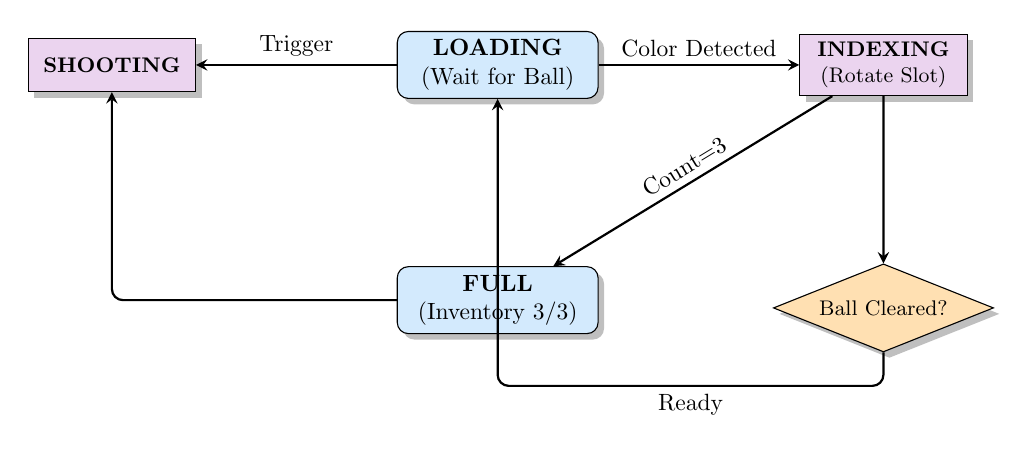
\begin{tikzpicture}[node distance=2.5cm, auto, scale=0.85, transform shape]
    % Nodes
    \node (loading) [process, text width=2.5cm] {\textbf{LOADING}\\(Wait for Ball)};
    \node (indexing) [action, right=3cm of loading] {\textbf{INDEXING}\\(Rotate Slot)};
    \node (wait) [decision, below=of indexing] {Ball Cleared?};
    \node (full) [process, below=of loading] {\textbf{FULL}\\(Inventory 3/3)};
    \node (shoot) [action, left=3cm of loading] {\textbf{SHOOTING}};
    
    % Flow Arrows
    \draw [arrow] (loading) -- node[above] {Color Detected} (indexing);
    \draw [arrow] (indexing) -- (wait);
    \draw [arrow] (wait.south) -- ++(0,-0.5) -| (loading.south) node[pos=0.25, below] {Ready};
    \draw [arrow] (loading) -- node[above] {Trigger} (shoot);
    \draw [arrow] (full) -| (shoot);
    \draw [arrow] (indexing) -- node[sloped, above] {Count=3} (full);
\end{tikzpicture}
\end{center}

\subsection{Motor Control: Velocity vs Power}
A critical lesson learned was the distinction between control modes.
\begin{itemize}
    \item \textbf{Shooter (RUN\_USING\_ENCODER):} Uses internal PID to maintain consistent RPM despite battery voltage drop.
    \item \textbf{Indexer (RUN\_TO\_POSITION):} Uses position PID to snap exactly to encoder targets (0, 96, 192...).
    \item \textbf{Intake (RUN\_WITHOUT\_ENCODER):} Simple voltage control for raw power.
\end{itemize}

\begin{lstlisting}[caption={Motor Mode Configuration}]
// Indexer: Position control for precision
indexer.setMode(DcMotor.RunMode.STOP_AND_RESET_ENCODER);
indexer.setTargetPosition(0);
indexer.setMode(DcMotor.RunMode.RUN_TO_POSITION);
indexer.setVelocityPIDFCoefficients(40, 5, 5, 10); // Custom Tuned PID

// Shooter: Velocity control for consistency
shooter.setMode(DcMotor.RunMode.RUN_USING_ENCODER);
\end{lstlisting}

\newpage
% ============================================================================
% SECTION 4: AUTONOMOUS & COMPUTER VISION
% ============================================================================
\section{Autonomous Navigation \& Vision}

\subsection{AprilTag Vision System}
We utilize the `AprilTagNavigator` class to provide absolute localization and game element detection.
\begin{enumerate}
    \item \textbf{Randomization Detection:} Scans IDs 21, 22, 23 (Obelisk) to determine the "Spike Mark" pattern.
    \item \textbf{Goal Alignment:} Scans ID 20 (Blue) or 24 (Red) for precise shooting alignment.
\end{enumerate}

\begin{lstlisting}[caption={AprilTag Proportional Navigation}]
// Calculate error signals
double rangeError = (desiredTag.ftcPose.range - DESIRED_DISTANCE);
double headingError = desiredTag.ftcPose.bearing;
double yawError = desiredTag.ftcPose.yaw;

// Apply proportional gains for corrective movement
double drive = Range.clip(rangeError * SPEED_GAIN, -MAX_SPEED, MAX_SPEED);
double turn = Range.clip(headingError * TURN_GAIN, -MAX_TURN, MAX_TURN);
double strafe = Range.clip(-yawError * STRAFE_GAIN, -MAX_STRAFE, MAX_STRAFE);
\end{lstlisting}

\subsection{Autonomous Flowchart (DecodeShootingAuto)}
The autonomous routine combines Roadrunner trajectories with our Smart Intake logic.

\begin{center}
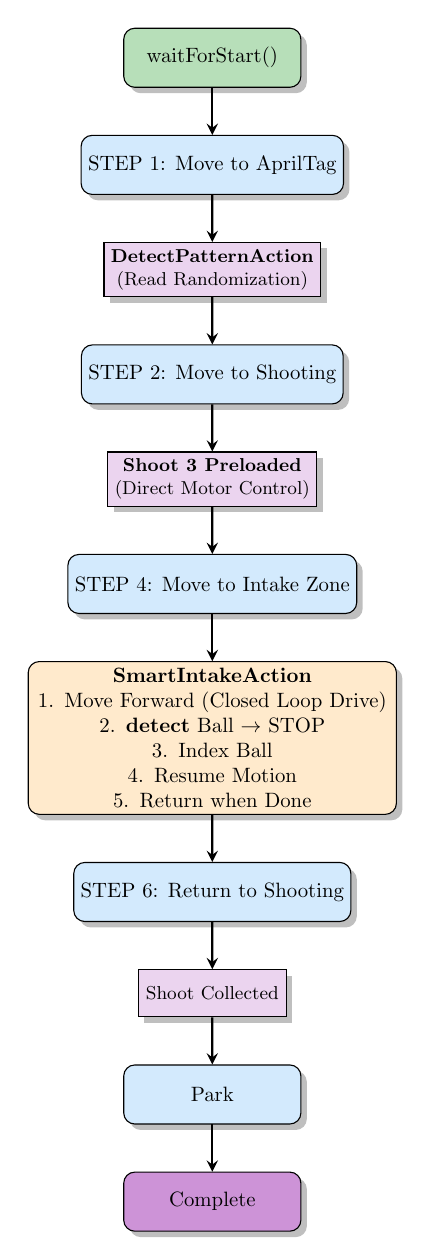
\begin{tikzpicture}[node distance=0.8cm, scale=0.75, transform shape]
    % Nodes - vertical flow
    \node (start) [startstop] {waitForStart()};
    \node (step1) [process, below=of start] {STEP 1: Move to AprilTag};
    \node (detect) [action, below=of step1] {\textbf{DetectPatternAction}\\(Read Randomization)};
    \node (step2) [process, below=of detect] {STEP 2: Move to Shooting};
    \node (step3) [action, below=of step2] {\textbf{Shoot 3 Preloaded}\\(Direct Motor Control)};
    \node (step4) [process, below=of step3] {STEP 4: Move to Intake Zone};
    
    % Smart Intake Complex Node
    \node (intake) [process, below=of step4, minimum height=2cm, fill=brandorange!20, text width=6cm] {
        \textbf{SmartIntakeAction}\\
        1. Move Forward (Closed Loop Drive)\\
        2. \textbf{detect} Ball $\rightarrow$ STOP\\
        3. Index Ball\\
        4. Resume Motion\\
        5. Return when Done
    };
    
    \node (step6) [process, below=of intake] {STEP 6: Return to Shooting};
    \node (step7) [action, below=of step6] {Shoot Collected};
    \node (step8) [process, below=of step7] {Park};
    \node (end) [startstop, below=of step8, fill=brandpurple!50] {Complete};
    
    % Arrows
    \draw [arrow] (start) -- (step1);
    \draw [arrow] (step1) -- (detect);
    \draw [arrow] (detect) -- (step2);
    \draw [arrow] (step2) -- (step3);
    \draw [arrow] (step3) -- (step4);
    \draw [arrow] (step4) -- (intake);
    \draw [arrow] (intake) -- (step6);
    \draw [arrow] (step6) -- (step7);
    \draw [arrow] (step7) -- (step8);
    \draw [arrow] (step8) -- (end);
\end{tikzpicture}
\end{center}

\subsection{Closed-Loop Drift Correction}
During the Smart Intake phase, the robot travels a long distance across tiles that may have variable friction. To prevent drift, we implemented a P-Controller that actively corrects heading and lateral deviation.

\textbf{Red Alliance Adaptation:}
A critical challenge was adapting this for the Red Alliance (mirrored).
$$ \text{Heading}_{red} = \text{Heading}_{blue} + 100^\circ $$
$$ \text{StrafeCorrection} = -1 \times K_p \times \text{Error} \quad (\text{Inverted sign due to 90 degree rotation}) $$

\begin{lstlisting}[caption={Drift Correction Logic}]
// Heading error
double headingError = targetHeading - currentPose.heading.toDouble();
// Normalize angle
while (headingError > Math.PI) headingError -= 2 * Math.PI;
while (headingError < -Math.PI) headingError += 2 * Math.PI;

// Corrections
double turnPower = headingError * headingKp;

// INVERTED for 90 deg heading (Red Alliance)
// At 90 deg, +Y strafe moves robot toward +X global
double strafeCorrection = -xError * strafeKp;  

drive.setDrivePowers(new PoseVelocity2d(
    new Vector2d(moveSpeed, strafeCorrection), turnPower));
\end{lstlisting}

\section{Summary of OpModes}
\begin{tabularx}{\textwidth}{|l|X|}
\hline
\textbf{OpMode} & \textbf{Description} \\
\hline
\textbf{A4 - Competition} & The main TeleOp. Combines Smart Auto-Indexing (A3) with AprilTag Driver Assist (A2). Includes "Share" button to toggle Red/Blue alliance targeting. \\
\hline
\textbf{DecodeShootingAuto} & Blue Alliance Autonomous. Full sequence: AprilTag $\rightarrow$ Shoot $\rightarrow$ Intake $\rightarrow$ Shoot $\rightarrow$ Park. \\
\hline
\textbf{DecodeShootingAutoRed} & Red Alliance Autonomous. Mirrored coordinates and inverted strafe correction logic. \\
\hline
\textbf{A3 - Smart Indexing} & TeleOp focused on the auto-indexing feature without vision assist. \\
\hline
\end{tabularx}

\end{document}
